%!TeX spellcheck = en_GB
\documentclass[conference]{IEEEtran}
\IEEEoverridecommandlockouts
% The preceding line is only needed to identify funding in the first footnote. If that is unneeded, please comment it out.
\usepackage{cite}
\usepackage{amsmath,amssymb,amsfonts}
\usepackage{algorithmic}
\usepackage{graphicx}
\usepackage{textcomp}
\usepackage{xcolor}

\begin{document}
	
	
	%refer the presentations/ notaability hints about writing a paper
	
	
	
	% describe the protocol for control access (blockchain part)
	%  Related work
	%	-   traditional architectures commenly employed in the IoT access:
	%	   XACML, OAuth, UMA
	%	   Dependency of a central entity
	
	% Our contribution should focus on the interoperability on the shared data, can be solved by BX view-update solution
	% 只是把receipt放在blockchain上(大家一起监督并达成一致性)
	%data放在自己出
	%dejima作为virtual,需要时产生
	
	%医生可以给病人提问题,然后病人回答,记录,因此data需要更新
	
	%优化access verification的措施 解决new authorization latency (like call-by-need)
	
	% 一旦一个新的node想发起访问,需要验证他的身份。
	% 但是一旦验证通过了之后,这个节点就被加入共享数据的白名单上,
	% 以后访问就不需要再验证了(即每次验证的时候先看whitelist上有没有这个用户,如果有,则直接有,则直接授权;否则需要大家完整验证)
	
	
	% describe the protocol for BX update procedure part

\title{Authorized Updates to Distributed Medical Data}

\author{
	\IEEEauthorblockN{%
		Chunmiao Li\textsuperscript{1},
		Yang Cao\textsuperscript{2},
		Zhenjiang Hu\textsuperscript{3},
		Masatoshi Yoshikawa\textsuperscript{4}
	\vspace{1.5ex}
	\IEEEauthorblockA{%
		\textsuperscript{1,\,3}\,National Institute of Informatics, Japan\qquad
		\textsuperscript{2,\,4}\,Kyoto University, Japan \\
		\textsuperscript{1,\,3}\,SOKENDAI (The Graduate University for Advanced Studies), Japan\qquad
		\textsuperscript{3}\,University of Tokyo, Japan
	}
	\vspace{1ex}
	\IEEEauthorblockA{%
		Email:\
		\textsuperscript{1}\,chunmiaoli1993@nii.ac.jp,
		\textsuperscript{2}\,yang@i.kyoto-u.ac.jp,
		\textsuperscript{3}\,hu@nii.ac.jp,
		\textsuperscript{4}\,yoshikawa@i.kyoto-u.ac.jp
	}
}
}

\maketitle

%规范下a, the, an 的使用
\begin{abstract}

% From MedRec: (our target problem)
% We recognize  that not all provider records can or should be made available to  patients (i.e. psychotherapy notes, or physician intellectual property) [6], and thus MedRec does not presume to be an automatic content-management system for all of a Physician's output. 我们更重要的是提出shared data和local data之间存在一致性关系
%MedRec does not claim to address the security of individual provider  databases where the record content is stored. (=> shared 部分也在其他peers中存一份) This must still be managed  by the local IT admin. Nor does MedRec attempt to solve the Digital  Rights Management problem. (data provider can 定制共享的数据 as view)

\end{abstract}

\begin{IEEEkeywords}
medical data, authorization, update
\end{IEEEkeywords}


%列一个文章每一部分怎么写的框架,参考论文写作课

\section{Introduction}

"Through the HIPAA Privacy Rule, providers can take
up to 60 days to respond (not necessarily to comply) to a request for updating or removing a record that
was erroneously added" \cite{centers2004hipaa}. 

"Interoperability challenges between different provider and hospital systems pose additional
barriers to effective data sharing. This lack of coordinated data management and exchange means health records are fragmented, rather than cohesive" \cite{mandl2001public}

"Patients benefit from a holistic, transparent picture of their medical history. In the age of online banking and social media, patients are increasingly willing, able and desirous of managing their data on the web and on the go [3]."\cite{mandl2001public}

"The ONC's report emphasizes that biomedical and public health researchers “require the ability to analyze information from many sources in order to identify public health risks, develop new treatments and cures, and enable precision medicine” \cite{office2015report}.

"We build on the work of Zyskind et al. \cite{zyskind2015decentralizing} to assemble references to data and encode these as hashed pointers onto a blockchain ledger. We then organize these references to explicitly create an accessible bread crumb trail for medical history, without storing raw medical data on the blockchain. " Our solution encodes the sharing peers in blockchain ledger and don't store the hash pointer to the raw data on ledger so that won't expose the privacy.

bidirectional transformation (BX hereafter)

We aims to solve problem update shared data between different peers. Since the shared data just reside in each peer's local database, read the shared data is easily promised.

But how about add, delete shared data?

We use two techniques to  solve a problem where blockchain is used to prevent malicious party to operate the 




%
%“Participants and health experts can then focus on individual health goals and questions, exchange knowledge to support individualized diagnoses and recommendations, and develop actionable and feasible plans to accommodate individual routines.
%
%Many clinics have begun to encourage patients to self-collect data that is traditionally collected by medical professionals, with the expectation of increasing clinic efficiency and promoting patient awareness.
%
%One example is the proliferation of self-service blood pressure kiosks. In a longitudinal, mixed-method study, I partnered with medical researchers to examine the adoption of self-service blood pressure kiosks in a family medicine clinic. Because of initial concerns raised by patients, staff, and clinicians, the clinic iteratively identified and addressed emerging challenges, provided timely solutions, and improved the overall workflow integration. 
%
%This work also provides a foundation for future researchers to study how personal informatics data can support management of other chronic diseases or preventive care, as well as how people with different expertise interact, communicate, and collaborate with each other.
% ”
% %分析师对数据的解释不就是修改/给医生提供的数据的解释和建议就是修改
% %医生可以根据病人的状况对药物信息作出调整,revise treatment plan
% %病人可以在共享的信息下查看解释后的记录,并且根据自己的状况更新健康数据给医生看
%

%Advantages of Medical data sharing
%
%However, health data are often sensitive and private and should be accessed under the permission of data owner.
%
%
%\textbf{The essentiality of update on sharing data.}
%
%According to the U.S. national health information privacy standards \cite{centers2003hipaa}, identifiable health information should not be exposed or just be accessed under the permission of patient or for public health practice.
%
%There are some requirements for medical data sharing:
%
%\begin{itemize}
%	\item Any operations on the shared data should be conducted after authorized (under the permission of patients).
%	\item Any modifications on the existing shared data should be updated to all sharing peers immediately.
%	\item Any access on medical data should be recorded.
%\end{itemize}
%
%Our contribution are as follow.
%
%\begin{enumerate}
%
%	\item  We identified the problems in medical data sharing (eg data privacy, transparency, lack of interoperability…) %我们识别出了共享数据和本地总数据之间的一致性关系
%	
%	\item  We surveyed existing blockchain-based solutions (eg. the three works you presented to us in the meeting) and clarify their disadvantages
%	
%	\item We discussed the essential components needed for medical data sharing  (but not been well studied in the literature )  and proposed our (visioned) solution to build a holistic solution utilizing blockchain.
%	
%	\item We proposed a decentralized medical data sharing architecture where data reside on owner's local database and metadata are stored on smart contract of  blockchain.
%	
%	
%	
%	
%\end{enumerate}

\section{Preliminary}

	\subsection{Blockchain}
	Proposed with Bitcoin \cite{nakamoto2008bitcoin} in 2008, blockchain technology has been widely used in many fields. Blockchain provides a solution for data storage, data transfer and consensus protocol in a distributed and decentralized environment. Generally speaking, blockchain is a shared ledger and replicated by all nodes on a distributed network, which records the historical valid transactions in a chronologically chained blocks. The nodes who generate new blocks via a proof-of-work are called miners.
	
	Not only can support the platform of cryptocurrency, blockchain can also be applied to other scenes. Ethereum \cite{wood2014ethereum} extend blockchain with additions such as a built-in Turing-complete programming language so that one can use this scripts (i.e., Ethereum Virtual Machine (EVM) byte codes) to write programs (i.e., smart contracts \footnote{Hyperledger and others still provide platforms to write smart contracts.}) on blockchain. We can just write Solidity \footnote{https://solidity.readthedocs.io/en/v0.5.2/} programs and then it can be compiled to EVM code. Besides the user accounts controlled by private keys like in Bitcoin, the accounts for smart contracts are allowed in Ethereum. Anyone can build decentralized applications which consists of a collection of smart contracts. Once a transaction involving smart contract creation gets confirmed, an address is generated for the contract and later anyone can send transactions to this address for executing the logic on it. A smart contract transaction is enforced when a miner includes it in a new produced block. Other nodes will validate it and re-run contracts if it is valid.
	
	\subsection{Bidirectional transformation}
	The theory of BXs was proposed to synchronize two parts of related information (i.e., source and view).  A BX consists of a pair of forward and backward transformations. A forward transformation (denoted as \emph{get}) extracts elements from the source to build an abstract view, and the backward transformation (denoted as \emph{put}\footnote{\emph{put} is not a simple inverse of \emph{get}. Instead, it accepts the view and the original source as input and produces an updated source as output.}) embeds information of the view back into the source and produces an updated source. This pair of transformations should satisfy the {\em round-tripping} laws (i.e., {\em well-behaveness}) called \emph{PutGet} and \emph{GetPut} properties. Specifically, \emph{GetPut} refers that no extra update should be performed back on the source when there is no change on the view, while \emph{PutGet} hints that \emph{put} should apply all changes on the view to the source so that the view can be regenerated from the updated source by \emph{get}. The most distinguished point of BX is that view can contain only a few part elements of source. Actually, BX stems from the the view update problem in database \cite{bancilhon1981update}, which studies how to translate the updates on a view table to the updates on the relating base (source) table. By designate some consistency between source and view, BX programs can synchronize the source and view and promise that they satisfy the consistency.
	
	One recent big progress towards practical use of BX is the observation that the essence of bidirectional programming is nothing but writing a well-behaved backward transformation (\emph{put})~\cite{hu2014validity, pacheco2014monadic, pacheco2014biflux}, because the corresponding forward transformation can be derived uniquely and freely. A core language, BiGUL~\cite{bigul}, has been developed for putback-based bidirectional programming.
    %refer BIRD
    
\section{System architecture}

In this section, we will illustrate our system architecture. Part A will describe the data distribution between sharing peers. Part B will present our system design and later explain it using an update scenario.

\subsection{Data distribution}

Shared data can exist in different peers, as shown in Fig. \ref{DB architecture}. Suppose there are three entities, doctor, researcher and patient. Doctor and Researcher share some data which are stored in D12 on Doctor side and D21 on researcher side respectively. D12 and D21 should contain the same data, which means if doctor or researcher update this shared data on their own side, then this modification should be propagated to the shared part on the other side. Accordingly, D13 and D31 have the same content and so do in D23 and D32.

Each node will store its all data on a bigger database, such as D1, D2 and D3. Each shared data can be seen as a view which is produced by this bigger database named as source. For example, D12 can be made from D1 by using \emph{get}. If D12 is modified, then the D1 need to be reproduced from original D1 and D12 by using \emph{put}. We just write BX in researcher and patient side to express the pair of \emph{get} and \emph{put} functions.

Note in our data distribution, shared data between any two parties will not be exposed to the third party, which can keep privacy between two parties in some degree. For example, any update on D12 and D21 can only be known by patient and researcher. However, after the change on D21 are reflected to D2, since D2 has been modified, D23 might need to be updated to a new version by using \emph{put} on D2.
%想表达任何两方共享数据的修改不会被第三方知道,但是对第三方数据的影响可以通过BX反映

Fig. \ref{dataRepresentation} presents an example to show data distribution between patient Alice, doctor Bob and researcher Charlie. Each party have their own local base table, named as D1, D2, D3 respectively. For each table, there are some attributes such as medication name and address on D1. Table D13 (also D31) are shared by Alice and Bob and can be produced from either D1 or D3 by \emph{get}. Table D23 (also D32) are shared by Charlie and Bob and can be generated from D2 or D3 by \emph{get}.  Shared tables all stay in sharing peer's local databases. Note here the metadata collection table resides in the smart contract on blockchain. Each entry of metadata collection table corresponds to a shared table. For example, the entry for D13 or D31 declare that it is shared by Alice and Bob and Bob can update all attributes value but Alice can only change the clinical data. The "Latest Update Time" shows when the metadata was changed most recently. Moreover, "Authority to Change Permission allow Bob to change other peers (here just Alice)'s authority so that Alice can update dosage by change the value for "Dosage" attribute to "Bob, Alice".

\begin{figure}[htbp]
	\centerline{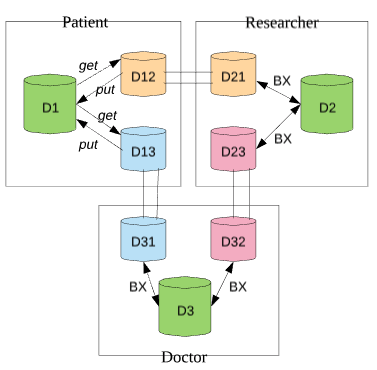
\includegraphics[width=250pt]{DBStructure.png}}
	\caption{DB architecture}
	\label{DB architecture}
\end{figure}

\begin{figure}[htbp]
	\centerline{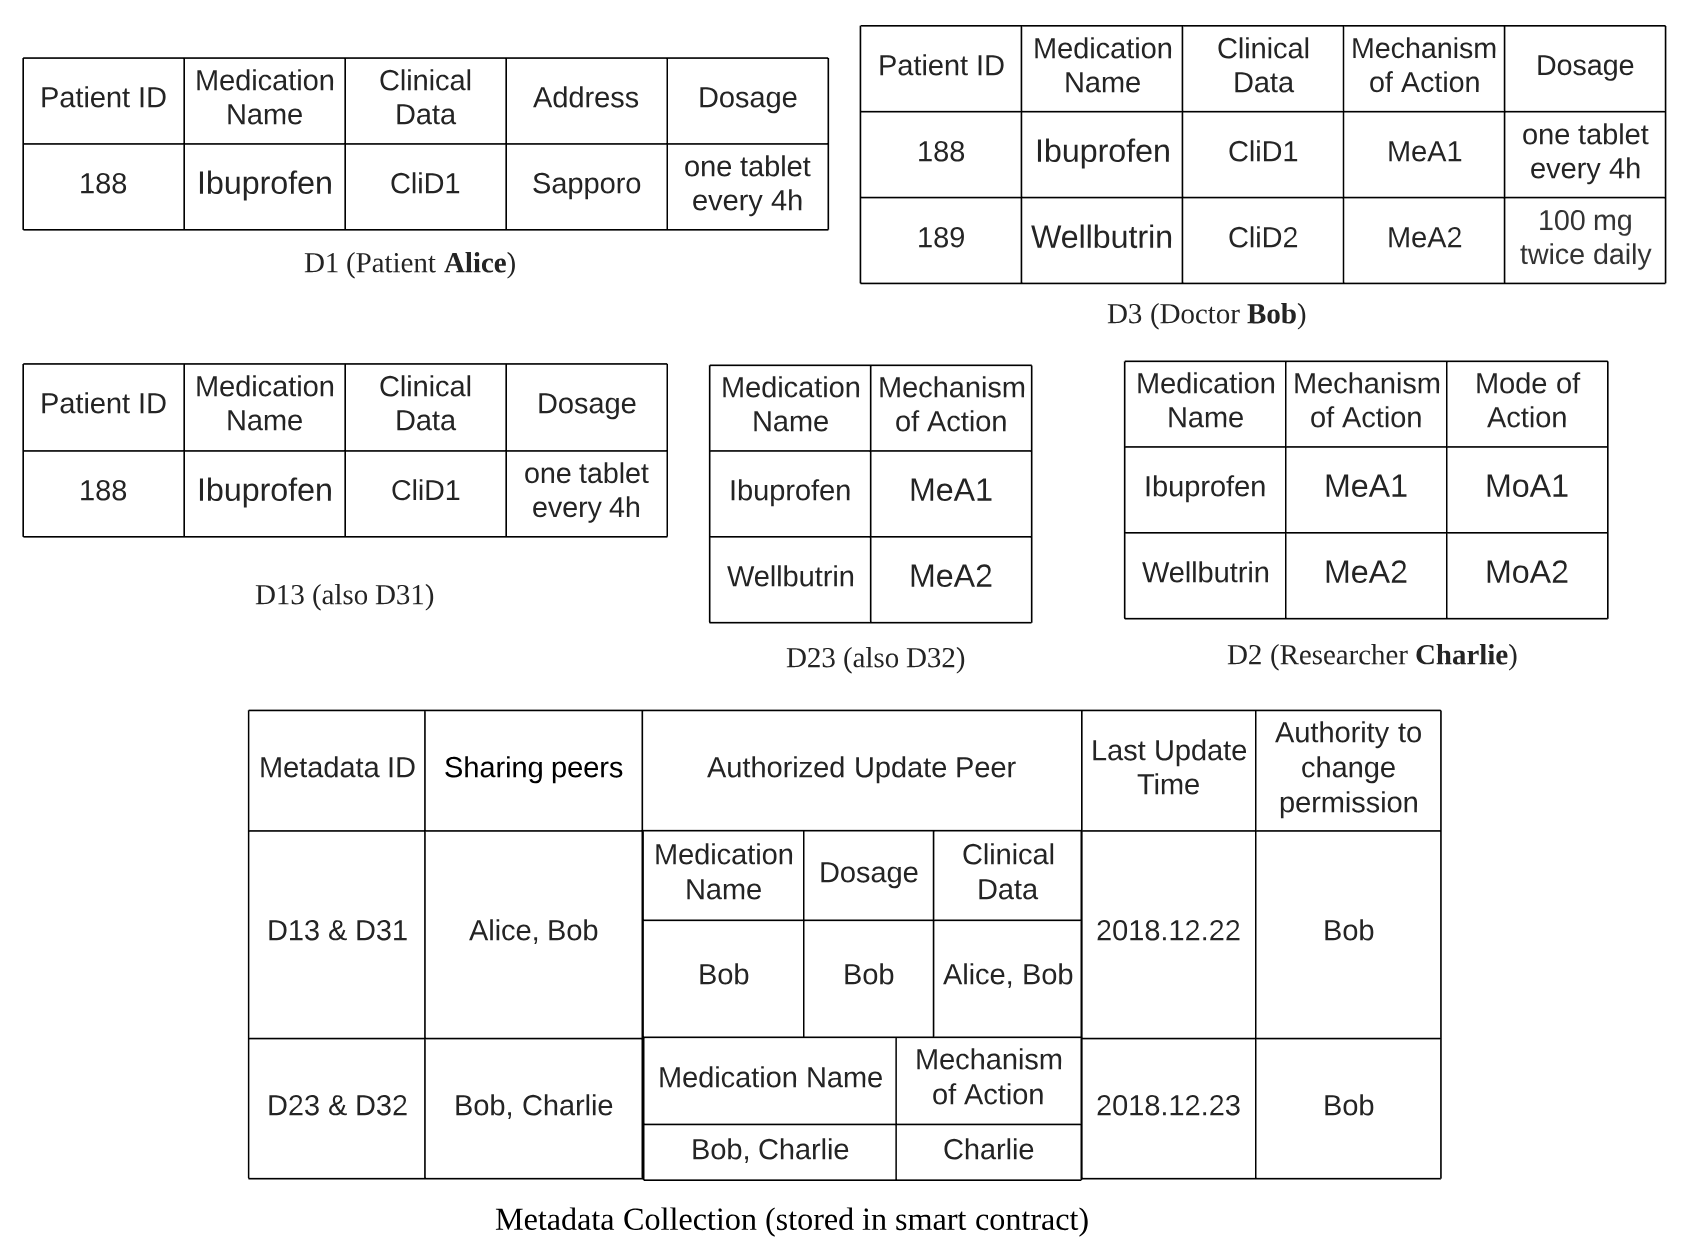
\includegraphics[width=250pt,height=220pt]{medicalData.png}}
	\caption{Data distribution}
	\label{dataRepresentation}
\end{figure}


\subsection{Permission on update data}
The metadata are created immediately once some peers wants to share data with each other. Suppose doctor Bob initiates the data sharing with Alice. He will deploy a smart contract on blockchain which stipulates the metadata about the shared data, such as sharing peers (i.e., Alice and Bob) and so on.  Table Metadata Collection on Fig. \ref{dataRepresentation} are built by Bob. 

Since smart contract can not be altered after it was deployed on blockchain. There are two ways to update the permission for update to shared data:
\begin{enumerate}
	\item deploy a new contract and notify all nodes on blockchain that this new one should be used to verify authority later;
	\item update the state of variables in contract.
\end{enumerate}
We choose the latter way. As shown in Fig. \ref{dataRepresentation}, the authority to modify the update permission are encoded in the field named as "authority to change permission". For example, for D13 and D31, Bob can change the permission to update "Dosage" to "Bob, Alice" so that Patient Alice can also update the  "Dosage".

\subsection{System design}
Our system consists of following components, which can be seen from Fig. \ref{workflow}.
\begin{itemize}
	\item Front-end user interface: control the interaction between users and other components.
	\item Database: each user has an overall database and many shared databases with other users. The latter can always be reproduced from the former.
	\item Blockchain: keep a record of access and update to the shared data. Also, fonrt-end user interface communicate with blockchain network via a blockchain node. The smart contract on blockchain contains the metadata of shared medical data and maintain an update log to store historical modification for each metadata.
	\item Database manager (server) dispose the synchronization between shared data and local data in terms of consistency logic relations.

\end{itemize}

\begin{figure}[htbp]
	\centerline{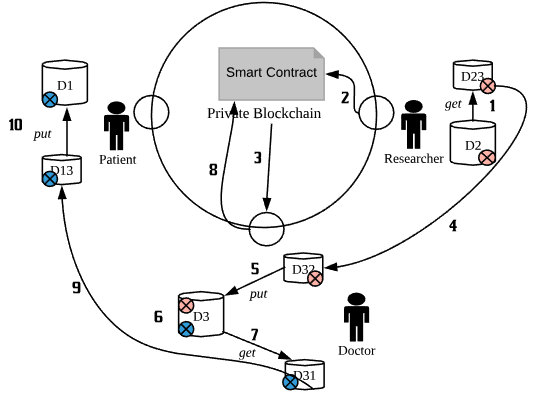
\includegraphics[width=230pt]{updateScenario.png}}
	\caption{An work flow for updating shared data}
	\label{workflow}
\end{figure}

\subsection{Case analysis}
Fig. \ref{workflow} depicts an scenario where researcher initiates the update the shared data. The numbers indicates the corresponding operations sequence.

After the update on D2, the researcher wants to propagate the update to the shared data D23 so that he uses the \emph{put} to regenerate D23 in(step 1). Then he will call a smart contract via a node by sending the repquest for update to the shared data (i.e., D32) (step 2). Note that a smart contract records all permission info about that shared data. Only the researcher's update satisfy the permission can his update be propagated to others. The smart contract will be executed until all nodes form consensus on this update request, which means researcher is authorized to update the shared data with doctor. Each node will conduct the smart contract locally. The metadata of shared data will be updated. Meanwhile, the node relating to Doctor will receive the notification from contract that the shared data with researcher need to modified (step 3). The doctor will request data from researcher by sending a message based on some encrypted communication protocol and get the newest shared data to refresh D32 (step 4). After that, doctor will use \emph{put} to reflect the change on D32 to the total database D3 (step 5). Since doctor shared some data (D31) with patient, he need to check whether D31 need to be reproduced (step 6). If yes, he will use \emph{get} to regenerate D31 (step 7) and request smart contract for permission to update D13 (step 8). Once this permission is allowed, patient will receive the notification about the change on shared data and ask doctor to send the updated D31. After patient get the modified D31 (step 9), he will use this to update D1 via \emph{put} (step 10).  

%Suppose a scenario as follow, which can be seen in Fig....
%
%Suppose Alice, Bob, Charlie are sharing data Da. 
%Alice update the local overall database and want to upload the update on the shared data. She will ask blockchain for permission. After the consensus, she should update the metadata of Da of smart contract on blockchain. Then smart contract will notify Bob and Charlie that the shared data has changed to a new version. Bob and Charlie will send request to Alice. Then Alice will apply \emph{get} to get the view (i.e., updated shared data) and send the Bob and  Charlie the new shared data. Once Bob or Charlie received the new Da, he will update the metadata on smart contract to show that he has upgrade the Da and then use \emph{put} to reflect the change on their own database. 
%
%%here like the orthogonal check on Ominzika sensei's picture
%Next Bob will check whether the update on local big DB will produce a new version of shared data with David. If yes, he will do the same procedure like Alice did at first.
%
%Only Alice, Bob, Charlie received the new Da, then the update on Da is successful. Else rollback???
%
%*************
%
%
%Still Bob need to whether he should update the dejima with David or others 
%
%Dependency 
%Incremental update
%Dependency graph
%
%Just send them data
%Put online; give them link
%Give data to each person
%
%Advantages of having data Locally not on server: 
%fast/easy to access
%Full control own data; change format
%exposed to others (since public available; sensitive data)
%scalability (multi access server; slow)


\section{discussion}

\subsection{Pros of our solution}
\begin{itemize}
	\item blockchain's distribute consensus protocol scheme keep the shared data between all sharing peers are consistent.
	
	\item Keep sensitive data private 
	%(MedRec: We recognize that not all provider records can or should be made available to patients (i.e. psychotherapy notes, or physician intellectual property) [6], and thus MedRec does not presume to be an automatic content-management system for all of a Physician's output. => We allow provider to designate the data want to share by giving consistent relationship)
	
	\item All modification on shared data can be recorded on blockchain (tamper-resist; permanent)
\end{itemize}

\subsection{Data source}
%"by integrating with providers' existing data storage infrastructure, we
%facilitate continued use of their existing systems. We believe this will ease adoption and aid compliance with HIPAA regulations. . In addition, MedRec is source agnostic, i.e. able to receive data from any number of endpoints (physician offices, hospital servers, patient home computers, et cetera). We have developed MedRec not as a proprietary system, but as a set of open APIs to facilitate EHR review and exchange. "

%\subsection{Maintaining the Integrity of the Specifications}

\subsection{Threat to validity}
\subsubsection{Privacy}
threat1 + possible solution
privacy: blockchain limitations 

\subsubsection{Throughput}
threat2 + possible solution

\subsubsection{Robustness}

\section{Related work}
The idea of introducing Blockchain technology to healthcare data system was presented firstly in \cite{yue2016healthcare} where they use blockchain for data storage to guarantee medical data can not be modified by anyone. Also, they designed a Healthcare Data Gateway (HDG) to control access of the shared data. However, medical data size can become huge so that become a burden for blockchain nodes' storage since each node have the same copy of blockchain. MedRec \cite{azaria2016medrec} choose to store raw medical data on providers' database and patients can download the data from it after authorized by smart contract on blockchain. They aimed to enable patient to engage in their healthcare.

But not all provider data such as physician intellectual property can be exposed to patients \cite{us2017individuals, grossman2011clinical}. Instead, we allow each node share a piece of medical data not total but still keep consistency between them after the updates to the shared ones. Additionally, any modifications on data shared by two nodes will not be disclosed to the third party which keep the consistency only exists in sharing peers. Moreover, since all shared data with others can be a part of each nodes' local total databases, we can decide whether one shared data have some influence on the other shared pieces and then propagate this change to the third party.

Our solution differs with previous ones. In our system, all parties, such as doctors, patients, and researchers can benefit from sharing data with others. 


\section{Conclusion}

In the future, we will use the real patient data to do experiment but use some de-identification technology to protect patient data from being exposed in terms of  

\section*{Acknowledgment}
The authors would like to thank all PRL lab members for the helpful advice in the draft version. 

\bibliographystyle{IEEEtran}
\bibliography{ref}

\end{document}
